\subsection{A Computer Map}
\label{sec:computer_map}

% Outcome: enumerate all the resources in a computer, understand what is shared

This section outlines the hardware components that make up a computer system
based on the Intel architecture.

\S~\ref{sec:motherboard} summarizes the structure of a \textit{motherboard}.
This is necessary background for reasoning about the cost and impact of
physical attacks against a computing system. \S~\ref{sec:intel_me} describes
Intel's Management Engine, which plays a role in the computer's bootstrap
process, and has significant security implications.

\S~\ref{sec:cpu_die} presents the building blocks of an Intel processor, and
\S~\ref{sec:cpu_core} models an Intel execution core at a high level. This is
the foundation for implementing defenses against physical attacks. Perhaps more
importantly, reasoning about software attacks based on information leakage,
such as timing attacks, requires understanding how a processor's computing
resources are shared and partitioned between mutually distrusting parties.

The information in here is either contained in the SDM or in Intel's
Optimization Reference Manual~\cite{intel2014optimization}.


\subsubsection{The Motherboard}
\label{sec:motherboard}

A computer's components are connected by a printed circuit board called a
\textit{motherboard}, shown in Figure~\ref{fig:motherboard}, which consists of
\textit{sockets} connected by \textit{buses}. Sockets connect chip-carrying
\textit{packages} to the board. The Intel documentation uses the term
``package'' to specifically refer to a CPU.

\begin{figure}[hbt]
  \centering
  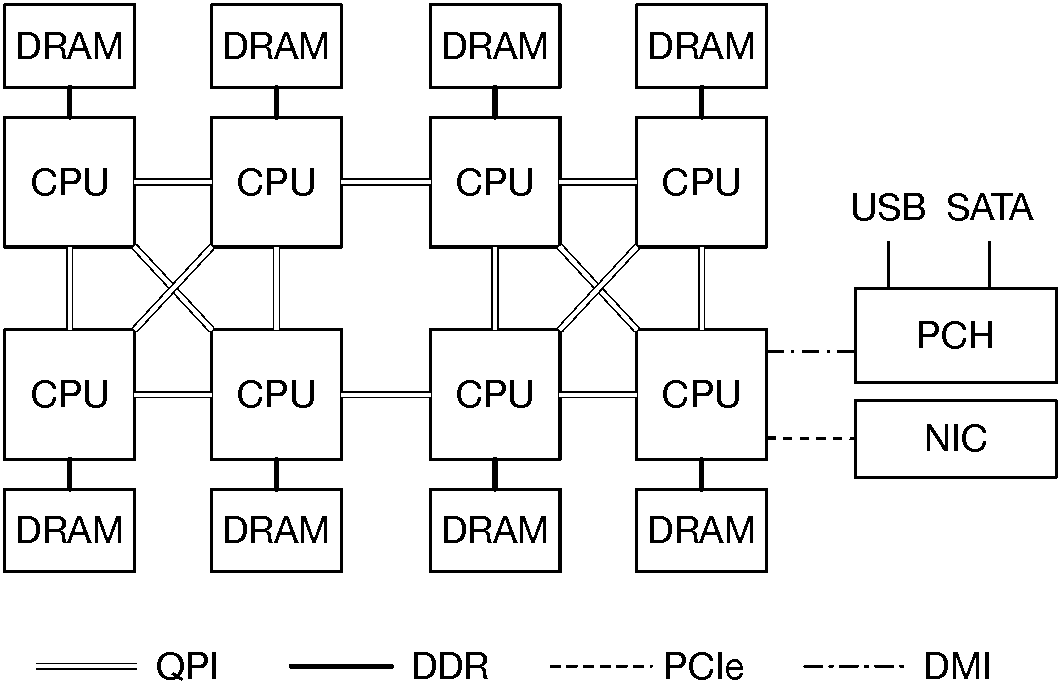
\includegraphics[width=85mm]{figures/motherboard.pdf}
  \caption{
    The motherboard structures that are most relevant in a system security
    analysis.
  }
  \label{fig:motherboard}
\end{figure}

The CPU (described in \S~\ref{sec:cpu_die}) hosts the execution cores that run
the SMM, hypervisor, operating system, and application software. The computer's
main memory is provided by \textit{Dynamic Random-Access Memory} (DRAM) chips.

The \textit{Platform Controller Hub}~(PCH) houses (relatively) low-speed I/O
controllers driving the slower buses in the system, like SATA, used by storage
devices, and USB, used by input peripherals. The PCH is also known as the
\textit{chipset}. At a first approximation, the \textit{south bridge} term in
older documentation can also be considered as a synonim for PCH.

Motherboards also have a non-volatile (flash) memory chip that hosts firmware
which implements the \textit{Unified Extensible Firmware Interface}~(UEFI)
specification~\cite{forum2015uefi}. The firmware contains the boot code and the
code that executes in System Management Mode (SMM, \S~\ref{sec:rings}).

The components we care about are connected by the following buses: the
\textit{Quick-Path Interconnect}~(QPI~\cite{intel2009qpi}), a network of
point-to-point links that connect processors, the
\textit{double data rate}~(DDR) bus that connects a CPU to DRAM, the
\textit{Direct Media Interface}~(DMI) bus that connects a CPU to the PCH, the
\textit{Peripheral Component Interconnect Express}~(PCIe) bus that connects
a CPU to peripherals such as a \textit{Network Interface Card}~(NIC), and the
\textit {Serial Programming Interface}~(SPI) used by the PCH to communicate
with the flash memory.

The PCIe bus is an extended, point-to-point version of the PCI standard, which
provides a method for any peripheral connected to the bus to perform
\textit{Direct Memory Access}~(DMA), transferring data to and from DRAM without
involving an execution core and spending CPU cycles. The PCI standard includes
a configuration mechanism that assigns a range of DRAM to each peripheral, but
makes no provisions for restricting a peripheral's DRAM accesses to its
assigned range.

Network interfaces consist of a \textit{physical} (PHY) module that converts
the analog signals on the network media to and from digital bits, and a
\textit{Media Access Control} (MAC) module that implements a network-level
protocol. Modern Intel-based motherboards forego a full-fledged NIC, and
instead include an Ethernet~\cite{ieee8023ethernet} PHY module.


\subsubsection{The Intel Management Engine (ME)}
\label{sec:intel_me}

Intel's \textit{Management Engine} (ME) is an embedded computer that was
initially designed for remote system management and troubleshooting of
server-class systems that are often hosted in data centers. However, all of
Intel's recent PCHs contain an ME~\cite{intel2013mefw}, and it currently plays
a crucial role in platform bootstrapping, which is described in detail in
\S~\ref{sec:booting}. Most of the information in this section is obtained from
an Intel-sponsored book~\cite{ruan2014intelme}.

The ME is part of Intel's \textit{Active Management Technology} (AMT), which is
marketed as a convenient way for IT administrators to troubleshoot and fix
situations such as failing hardware, or a corrupted OS installation, without
having to gain physical access to the impacted computer.

The Intel ME, shown in Figure~\ref{fig:intel_me}, remains functional during
most hardware failures because it is an entire embedded computer featuring its
own execution core, bootstrap ROM, and internal RAM. The ME can be used for
troubleshooting effectively thanks to an array of abilities that include
overriding the CPU's boot vector and a DMA engine that can access the
computer's DRAM. The ME provides remote access to the computer without any CPU
support because it can use the \textit{System Management bus} (SMBus) to access
the motherboard's Ethernet PHY, or an AMT-compatible NIC
\cite{intel2015chipset}.

\begin{figure}[hbt]
  \centering
  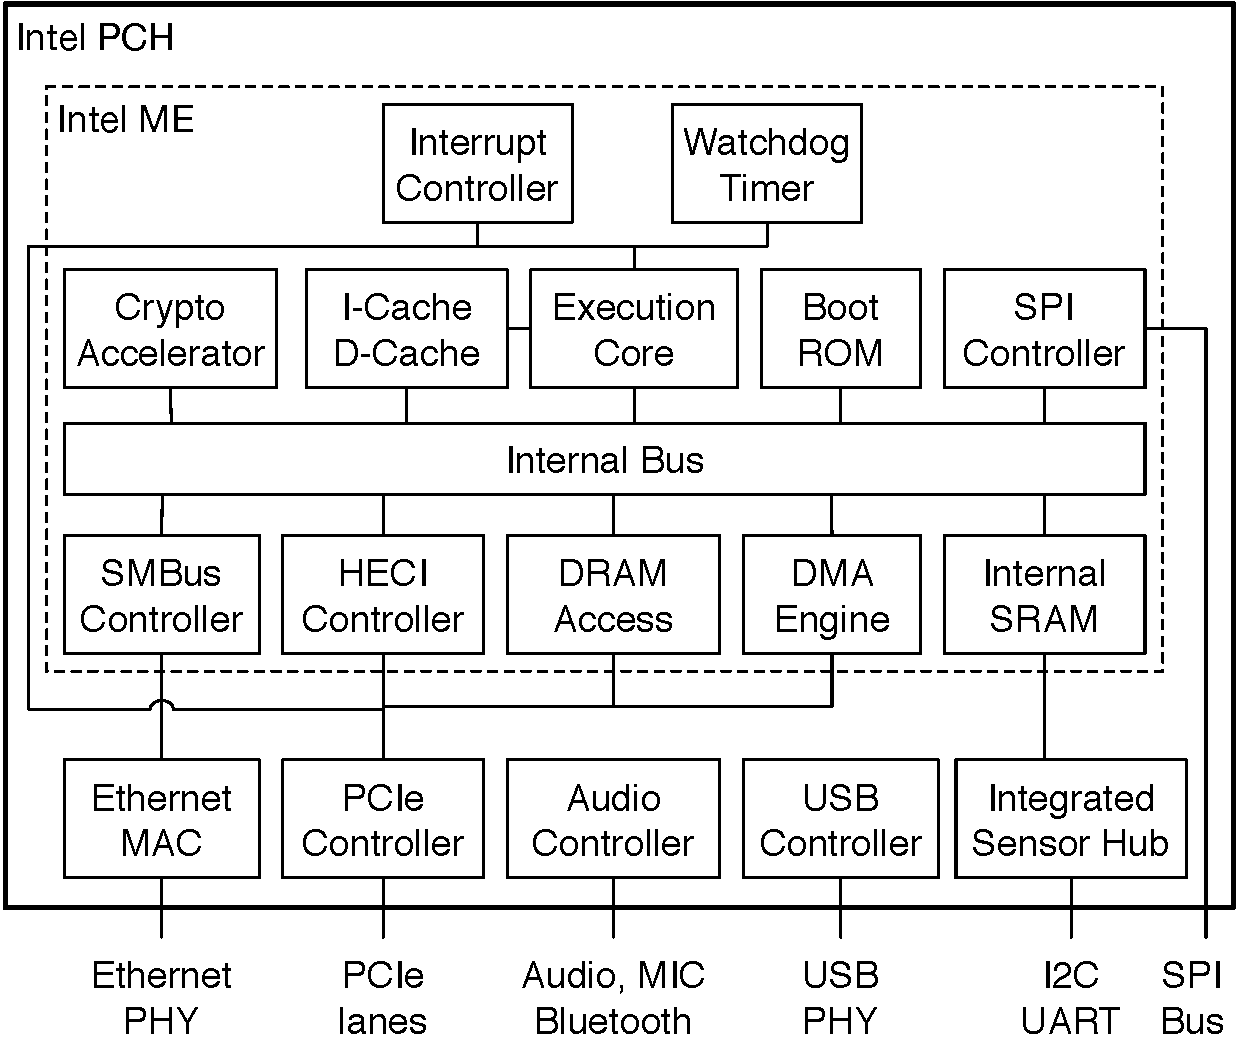
\includegraphics[width=85mm]{figures/intel_me.pdf}
  \caption{
    The Intel Management Engine (ME) is an embedded computer hosted in the
    PCH. The ME has its own execution core, ROM and SRAM. The ME can access the
    host's DRAM via a memory controller and a DMA controller. The ME is
    remotely accessible over the network, as it has direct access to an
    Ethernet PHY via the SMBus.
  }
  \label{fig:intel_me}
\end{figure}

% Power and Ground Signals: Series 100 Chipset datasheet S 8
% PCH and System Power States: Series 100 Chipset datasheet S 26.7.2

The Intel ME is connected to the motherboard's power supply using a power rail
that stays active even when the host computer is in the \textit{Soft Off} mode
\cite{intel2015chipset}, known as ACPI G2/S5, where most of the computer's
components are powered off \cite{intel2010power}, including the CPU and DRAM.
For all practical purposes, this means that the ME's execution core is active
as long as the power supply is still connected to a power source.

In S5, the ME cannot access the DRAM, but it can still use its internal
memories. The ME can also still communicate with a remote party, as it can
access the motherboard's Ethernet PHY via SMBus. This enables applications such
as AMT's theft prevention, where a laptop equipped with a cellular modem can be
tracked and permanently disabled as long as it has power and signal.

As the ME remains active in deep power-saving modes, its design must rely on
low-power components. The execution core is Argonaut RISC Core (ARC) clocked at
200-400Mhz, which is typically used in low-power embedded designs. On a very
recent PCH \cite{intel2015chipset}, the internal SRAM has 640KB, and is shared
with the Integrated Sensor Hub (ISH)'s core. The SMBus runs at 1Mhz and,
without CPU support, the motherboard's Ethernet PHY runs at 10Mpbs.

When the host computer is powered on, the ME's execution core starts running
code from the ME's bootstrap ROM. The bootstrap code loads the ME's software
stack from the same flash chip that stores the host computer's firmware. The
ME accesses the flash memory chip an embedded SPI controller.


\subsubsection{The Processor}
\label{sec:cpu_die}

An Intel processor's die, illustrated in Figure~\ref{fig:cpu_die}, is divided
into two broad areas: the \textit{core area} implements the instruction
execution pipeline typically associated with CPUs, while the \textit{uncore}
provides functions that were traditionally hosted on separate chips, but are
currently integrated on the CPU die to save power and improve latency.

\begin{figure}[hbt]
  \centering
  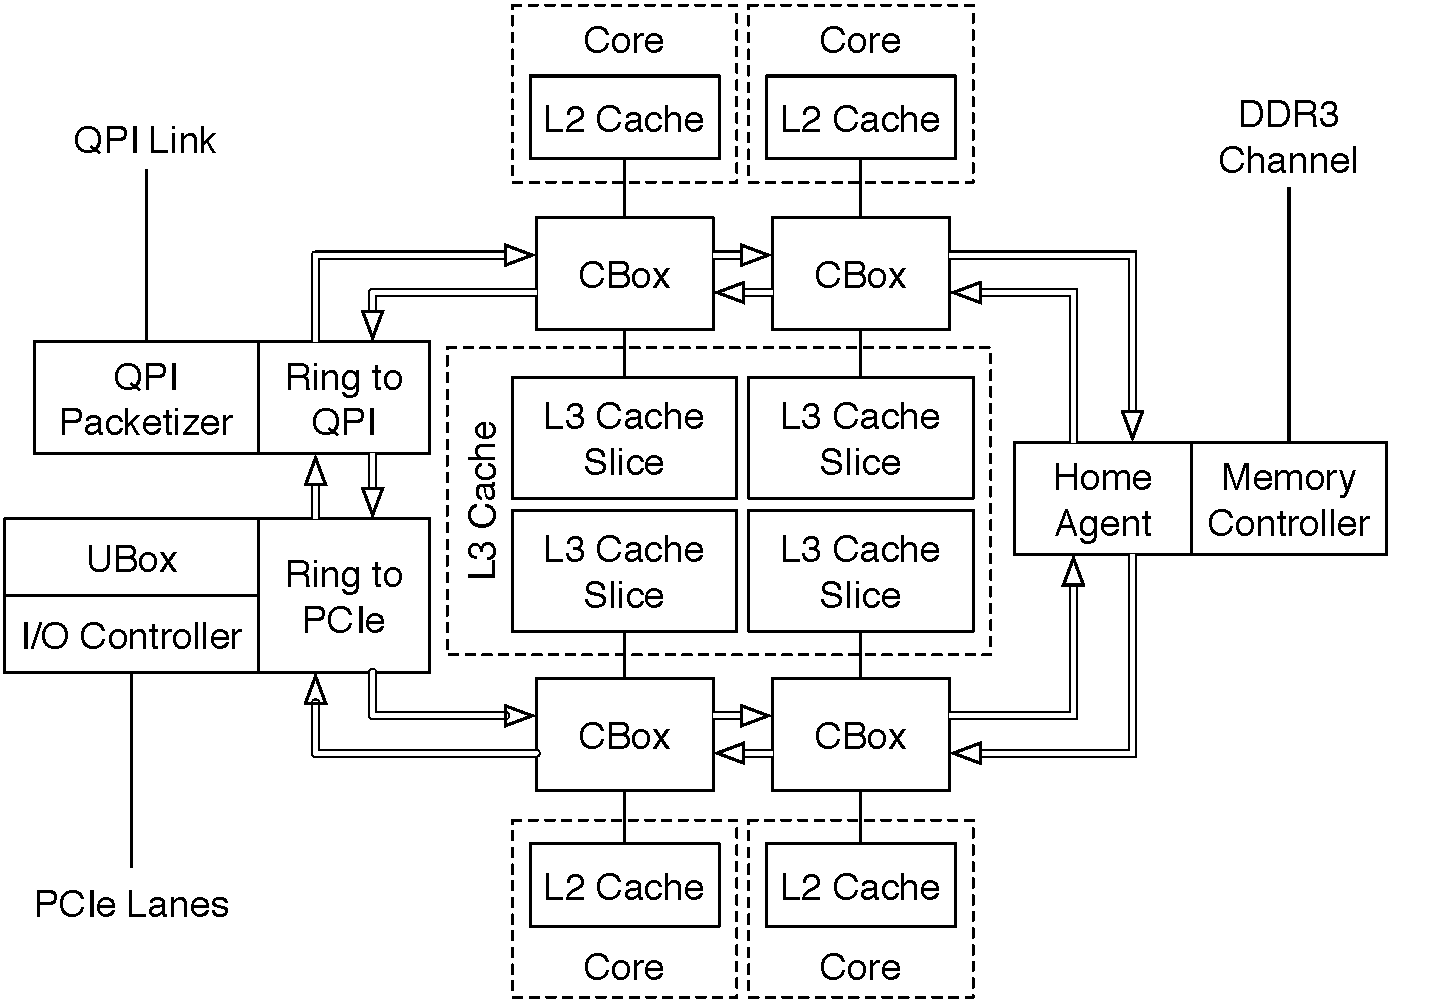
\includegraphics[width=85mm]{figures/cpu_die.pdf}
  \caption{
    The major components in a modern CPU package. \S~\ref{sec:cpu_die} gives
    an uncore overview. \S~\ref{sec:cpu_core} describes execution cores.
    \S~\ref{sec:cache_coherence} takes a deeper look at the uncore.
  }
  \label{fig:cpu_die}
\end{figure}

% Ring Interconnect and Last Level Cache: Optimization S 2.2.5.3
% System Agent: Optimization S 2.2.6

At a conceptual level, the uncore of modern processors includes an
\textit{integrated memory controller} (iMC) that interfaces with the DDR bus,
an \textit{integrated I/O controller} (IIO) that implements PCIe bus lanes and
interacts with the DMI bus, and a growing number of integrated peripherals,
such as a \textit{Graphics Processing Unit} (GPU). The uncore structure is
described in some processor family datasheets \cite{intel2014datasheet,
intel2010datasheet}, and in the overview sections in Intel's uncore performance
monitoring documentation \cite{intel2014uncore, intel2012uncore,
intel2010uncore}.

Security extensions to the Intel architecture, such as Trusted Execution
Technology~(TXT)~\cite{grawrock2009txt} and Software Guard
Extensions~(SGX)~\cite{mckeen2013sgx, anati2013sgx}, rely on the fact that the
processor die includes the memory and I/O controller, and thus can prevent any
device from accessing protected memory areas via \textit{Direct Memory Access}
(DMA) transfers. \S~\ref{sec:cache_coherence} takes a deeper look at the uncore
organization and at the machinery used to prevent unauthorized DMA transfers.


\subsubsection{The Core}
\label{sec:cpu_core}

Virtually all modern Intel processors have core areas consisting of multiple
copies of the execution core circuitry, each of which is called a
\textit{core}.  At the time of this writing, desktop-class Intel CPUs have 4
cores, and server-class CPUs have as many as 18 cores.

Most Intel CPUs feature \textit{hyper-threading}, which means that a core
(shown in Figure~\ref{fig:cpu_core}) has two copies of the register files
backing the execution context described in \S~\ref{sec:registers}, and can
execute two separate streams of instructions simultaneously. Hyper-threading
increases the utilization of the shared fetch, decode and execution units, in
the presence of memory stalls.

\begin{figure}[hbt]
  \centering
  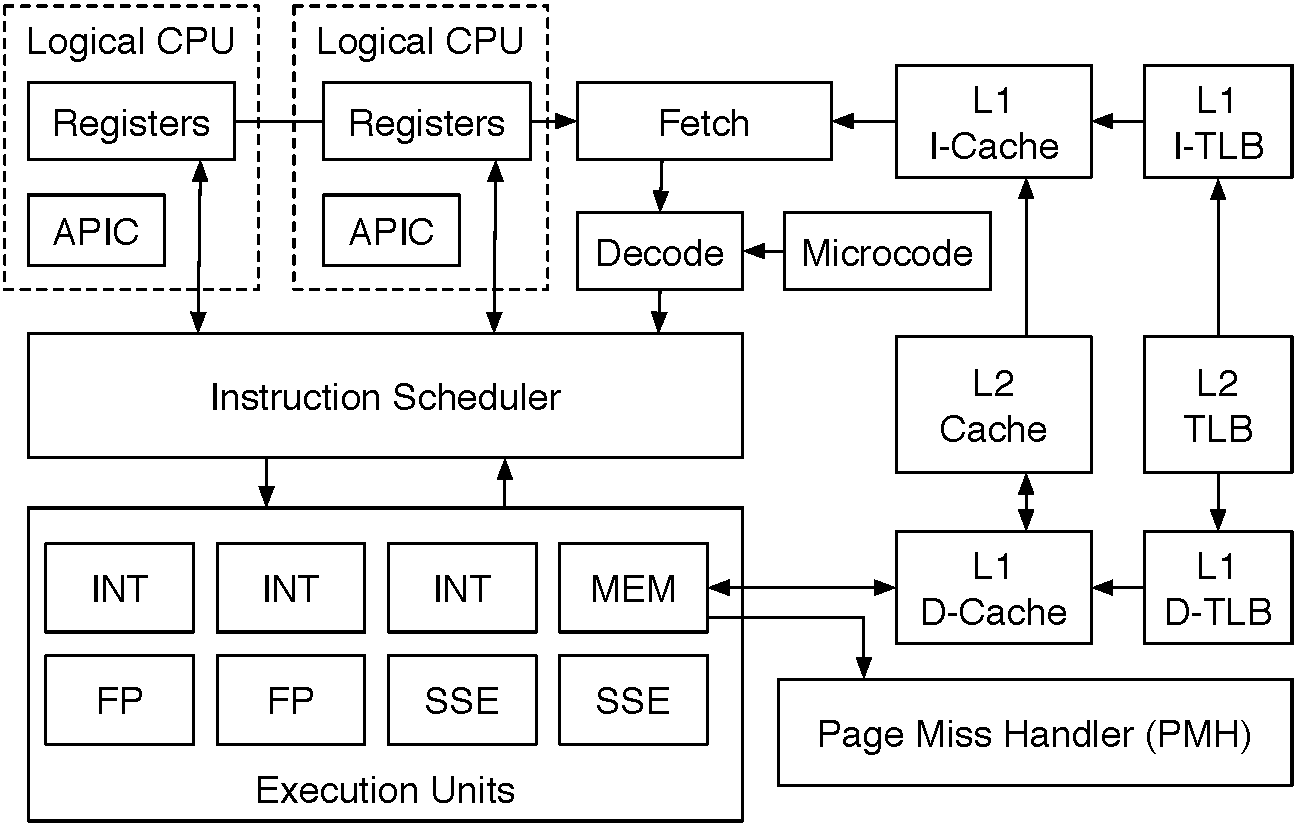
\includegraphics[width=85mm]{figures/cpu_core.pdf}
  \caption{
    CPU core with two logical processors. Each logical processor has its own
    execution context and LAPIC (\S~\ref{sec:interrupts}). All the other core
    resources are shared.
  }
  \label{fig:cpu_core}
\end{figure}

A hyper-threaded core is exposed to system software as two \textit{logical
processors}~(LPs), also named \textit{hardware threads} in the Intel
documentation. The logical processor abstraction allows the code used to
distribute work across processors in a multi-processor system to function
without any change on multi-core hyper-threaded processors.

The high level of resource sharing introduced by hyper-threading introduces a
security vulnerability. Software running on one logical processor can use the
high-resolution performance counter (\texttt{RDTSCP},
\S~\ref{sec:address_spaces}) \cite{petters1999making} to get information about
the instructions and memory access patterns of another piece of software that
is executed on the other logical processor on the same core.
